\chapter{Outils mathématiques d'ordre général}
\begin{spacing}{1.2}
\minitoc
\thispagestyle{MyStyle}
% \setstretch{1.2} 
\end{spacing}
\newpage
\justifying

\sloppy \setstretch{1.3} 
\section{Introduction}

Ce chapitre couvre les techniques de prétraitement, les tests de corrélation et la modélisation. Nous abordons des méthodes comme la normalisation et le traitement des valeurs manquantes, puis explorons des outils statistiques pour analyser les relations entre variables. Enfin, nous présentons des techniques de modélisation, incluant l’équilibrage des classes et la sélection de caractéristiques, qui améliorent les performances des modèles prédictifs.

\section{Techniques de Prétraitement des Données}

Le prétraitement des données est une étape cruciale pour améliorer la qualité des données et optimiser les performances des modèles. Il inclut des méthodes comme la normalisation, qui ajuste l'échelle des variables, et le traitement des valeurs manquantes.

\subsection{Normalisation des Données}

La normalisation met toutes les variables sur une même échelle, ce qui est essentiel pour éviter qu'une variable domine en raison de son amplitude. C’est particulièrement utile pour les algorithmes sensibles à l'échelle des données.

\subsubsection{Méthodes classiques de normalisation}

\textbf{\(\checkmark\)} \textbf{Normalisation Min-Max} \\
Elle met les données à l’échelle entre 0 et 1 selon la formule suivante: 
    \[
    X_{\text{norm}} = \frac{X - X_{\text{min}}}{X_{\text{max}} - X_{\text{min}}}
    \]
\textbf{\(\rightarrow\)} \textbf{Utilité}: Recommandée pour les algorithmes comme les réseaux de neurones.\\
\textbf{\(\rightarrow\)} \textbf{Impact}: Sensible aux valeurs extrêmes (outliers).

\textbf{\(\checkmark\)} \textbf{Z-Score (Standardisation)} \\
    Cette méthode centre les données à 0 avec un écart-type de 1 selon la formule suivante:
    \[
    X_{\text{std}} = \frac{X - \mu}{\sigma}
    \]
\textbf{\(\rightarrow\)} \textbf{Utilité}: Utile pour ajuster les échelles sans affecter la structure des variables, peu importe la distribution.\\
\textbf{\(\rightarrow\)} \textbf{Impact}: Uniformise l'effet des variables sur le modèle.

\textbf{\(\checkmark\)} \textbf{Normalisation Logarithmique (Log)} \\
    La transformation logarithmique réduit l'influence des grandes valeurs et rend les distributions plus symétriques selon la formule suivante: 
    \[
    X_{\text{log}} = \log(X + 1)
    \]
\textbf{\(\rightarrow\)} \textbf{Utilité}: Efficace pour réduire les écarts dus aux valeurs extrêmes.\\
\textbf{\(\rightarrow\)} \textbf{Impact}: Diminue l'influence des grandes valeurs.

\textbf{\(\checkmark\)} \textbf{Transformation par Racine Carrée (Sqrt)} \\
    Cette transformation réduit la variance tout en préservant la hiérarchie des données. Formule :
    \[
    X_{\text{sqrt}} = \sqrt{X}
    \]
\textbf{\(\rightarrow\)} \textbf{Utilité}: Réduit l'impact des grandes valeurs sans affecter l'ordre des données.\\
\textbf{\(\rightarrow\)} \textbf{Impact}: Atténue les grandes variations tout en maintenant la structure des données.

\subsubsection{Méthodes avancées de normalisation}

Pour améliorer la qualité des données, surtout lorsque celles-ci ne suivent pas une distribution normale, des techniques avancées comme la transformation de Box-Cox et la transformation de Yeo-Johnson sont souvent employées.

\textbf{\(\checkmark\)} \textbf{Transformation de Box-Cox} \\
La transformation de Box-Cox stabilise la variance et rapproche les données d'une distribution normale. Elle est définie par:

\[
y(\lambda) =
\begin{cases} 
\frac{x^\lambda - 1}{\lambda}, & \text{si } \lambda \neq 0 \\
\log(x), & \text{si } \lambda = 0
\end{cases}
\]

\noindent \textbf{\(\rightarrow\)} \textbf{Explication}: Box-Cox applique une transformation exponentielle ou logarithmique aux données, selon la valeur de $\lambda$. Lorsque $\lambda$ est différent de zéro, la transformation lisse les données et réduit l'asymétrie en modifiant la relation entre les valeurs observées et la moyenne. Si $\lambda = 0$, elle applique une transformation logarithmique pour atténuer l'impact des grandes valeurs tout en rendant la distribution plus symétrique. Nous approfondirons la notion de \textbf{log-vraisemblance} dans une section ultérieure.\\
\textbf{\(\rightarrow\)} \textbf{Utilité}: Utile pour les données strictement positives, permet d'uniformiser les distributions non normales.\\
\textbf{\(\rightarrow\)} \textbf{Choix de $\lambda$}: Le paramètre $\lambda$ est choisi par maximisation de la log-vraisemblance.

\textbf{\(\checkmark\)} \textbf{Transformation de Yeo-Johnson} \\
Cette transformation est une généralisation de Box-Cox qui permet de traiter à la fois les données positives et négatives. Elle est définie par:

\[
y(\lambda) =
\begin{cases} 
\frac{(x + 1)^\lambda - 1}{\lambda}, & \text{si } \lambda \neq 0 \text{ et } x \geq 0 \\
\log(x + 1), & \text{si } \lambda = 0 \text{ et } x \geq 0 \\
-\frac{(-x + 1)^{2 - \lambda} - 1}{2 - \lambda}, & \text{si } \lambda \neq 2 \text{ et } x < 0 \\
-\log(-x + 1), & \text{si } \lambda = 2 \text{ et } x < 0
\end{cases}
\]

\noindent \textbf{\(\rightarrow\)} \textbf{Utilité}: Permet de traiter les données négatives et positives, rendant les données plus normalisées.\\
\textbf{\(\rightarrow\)} \textbf{Choix de $\lambda$}: Comme pour Box-Cox, $\lambda$ est déterminé par maximisation de la log-vraisemblance.

\subsection{Traitement des Valeurs Manquantes}

Le traitement des valeurs manquantes est crucial pour maintenir la qualité des modèles prédictifs. Il permet d'éviter les biais introduits par des données incomplètes en remplaçant les valeurs manquantes par des estimations appropriées.

\subsubsection{Imputation par la Médiane}

L’imputation par la médiane est une méthode simple qui remplace les valeurs manquantes par la médiane de la variable concernée. Elle est particulièrement efficace pour les données avec des valeurs extrêmes (outliers), car la médiane n'est pas influencée par ces dernières.

\[
x_{i,\text{missing}} = \text{Médiane}(x_i)
\]

\noindent \textbf{\(\rightarrow\)} \textbf{Utilité}: Adaptée aux distributions asymétriques.\\
\textbf{\(\rightarrow\)} \textbf{Impact}: Remplace les valeurs manquantes sans perturber la distribution des données.

\subsubsection{K-Nearest Neighbors pour la Prédiction des Valeurs Manquantes}

Le K-Nearest Neighbors (KNN) repose sur la similarité des données pour imputer les valeurs manquantes. Il identifie les \(k\) voisins les plus proches de l'observation avec la valeur manquante, en se basant sur une mesure de distance. Parmi ces mesures, la distance de Minkowski est une généralisation couramment utilisée.

\textbf{\(\checkmark\)} \textbf{Étape 1: Calcul de la distance de Minkowski:} \\
La distance de Minkowski est définie par :

\[
d(x_i, x_j) = \left( \sum_{k=1}^{n} |x_{ik} - x_{jk}|^p \right)^{1/p}
\]

\textbf{Cas particuliers:}\\
\textbf{\(\rightarrow\)} Si \( p = 2 \), on obtient la \textbf{distance euclidienne}, utilisée pour les données continues.\\
\textbf{\(\rightarrow\)} Si \( p = 1 \), on obtient la \textbf{distance de Manhattan}, adaptée aux données avec de grandes variations.\\
\textbf{\(\rightarrow\)} Pour d'autres valeurs de \( p \), la \textbf{distance de Minkowski} offre une flexibilité accrue pour ajuster la mesure de similarité.

\noindent \textbf{\(\rightarrow\)} \textbf{Utilité}: Chaque type de distance est choisi en fonction de la nature des données.\\
\textbf{\(\rightarrow\)} \textbf{Impact}: Le choix de la distance influence les voisins sélectionnés, et donc la précision de l'imputation.

\textbf{\(\checkmark\)} \textbf{Étape 2: Moyenne pondérée des voisins:} \\
Une fois les voisins identifiés, la valeur manquante est imputée par une moyenne pondérée de leurs valeurs :

\[
x_{i,\text{missing}} = \frac{\sum_{j \in N(i)} w_j x_j}{\sum_{j \in N(i)} w_j}
\]

où \(w_j\) est un poids inversement proportionnel à la distance \(d(x_i, x_j)\).

\noindent \textbf{\(\rightarrow\)} \textbf{Utilité}: Produit des estimations plus précises que les méthodes simples.\\
\textbf{\(\rightarrow\)} \textbf{Impact}: Les valeurs imputées sont souvent plus proches des vraies données manquantes, augmentant la précision des modèles.

\subsection{Conclusion}

Le prétraitement, notamment la normalisation et le traitement des valeurs manquantes, est essentiel pour garantir des données comparables et fiables, améliorant ainsi les performances des modèles prédictifs.

\section{Les indicateurs statistiques}

Les \textbf{indicateurs statistiques} résument les données et permettent de mesurer les relations entre variables. Parmi eux, on trouve:\\

\noindent  \textbf{\(\rightarrow\)} \textbf{Tendance centrale :} Moyenne, médiane, mode indiquent où se concentrent les valeurs.\\
\textbf{\(\rightarrow\)} \textbf{Dispersion :} Variance, écart-type et étendue quantifient la variabilité autour de la tendance centrale.\\
\textbf{\(\rightarrow\)} \textbf{Relation :} Covariance et coefficient de corrélation mesurent les relations linéaires entre variables quantitatives.\\
\textbf{\(\rightarrow\)} \textbf{Association :} L’Eta carré et le Cramer V évaluent l’association entre variables.

\subsection{Eta Carré}

L'Eta carré (\(\eta^2\)) quantifie la part de variance d'une variable quantitative expliquée par une variable qualitative. Il mesure l'effet d'un facteur.

\[
\eta^2 = \frac{SSB}{SSB + SSW}
\]

Avec :
\begin{itemize}
    \item \( SSB \) : Somme des Carrés Entre les Groupes, mesurant la différence entre les moyennes des groupes et la moyenne générale.
    \item \( SSW \) : Somme des Carrés Intra-Groupes, mesurant la variabilité à l'intérieur de chaque groupe.
\end{itemize}

\textbf{\(\checkmark\)} \textbf{Interprétation}:\\
\noindent \textbf{\(\rightarrow\)} \(\eta^2 \leq 0.01\) : Effet faible.\\
\textbf{\(\rightarrow\)} \(0.01 < \eta^2 \leq 0.06\) : Effet modéré.\\
\textbf{\(\rightarrow\)} \(\eta^2 > 0.06\) : Effet fort.

\subsection{Cramer V}

Le \textbf{Cramer V} mesure la force de l'association entre deux variables qualitatives, basé sur la statistique du \(\chi^2\). Il est souvent utilisé avec un \textbf{tableau de contingence}, qui montre la fréquence des combinaisons possibles entre deux variables catégorielles. On détaillera ce tableau et le calcul du \(\chi^2\) dans une prochaine section.

\[
V = \sqrt{\frac{X^2}{N \times \min(k-1, r-1)}}
\]

Où:
\begin{itemize}
    \item \(X^2\) est la statistique du \(\chi^2\),
    \item \(N\) est le nombre total d’observations,
    \item \(k\) et \(r\) sont respectivement le nombre de colonnes et de lignes dans le tableau de contingence.
\end{itemize}

\textbf{\(\checkmark\)} \textbf{Interprétation}: \\
\noindent \textbf{\(\rightarrow\)} $V \leq 0.10$: Association faible.\\
\textbf{\(\rightarrow\)} $0.10 < V \leq 0.30$: Association modérée.\\
\textbf{\(\rightarrow\)} $V > 0.30$: Forte association.

\subsection{Lambda de Goodman et Kruskal}

Le \textbf{Lambda} (\(\lambda\)) mesure l'amélioration de la prédiction d'une variable qualitative dépendante en fonction d'une variable qualitative indépendante. Il compare les erreurs de prédiction avec et sans la variable indépendante.
\[
\lambda = \frac{E_0 - E_1}{E_0}
\]

Où:
\begin{itemize}
    \item \(E_0 = N - \max_j(n_j)\) est le nombre d'erreurs si l'on prédit toujours la modalité la plus fréquente de la variable dépendante (erreurs sans utiliser la variable indépendante),
    \item \(E_1 = \sum_{i} \left( n_i - \max_j \left( n_{ij} \right) \right)\) est le nombre d'erreurs en utilisant la variable indépendante pour prédire la variable dépendante.
\end{itemize}

\textbf{\(\checkmark\)} \textbf{Interprétation}:\\
\noindent \textbf{\(\rightarrow\)} \( \lambda \leq 0.10 \): Amélioration faible.\\
\textbf{\(\rightarrow\)}  \( 0.10 < \lambda \leq 0.30 \): Amélioration modérée.\\
\textbf{\(\rightarrow\)}  \( \lambda > 0.30 \): Amélioration significative.

\subsection{Covariance}

La \textbf{covariance} mesure la variation conjointe de deux variables quantitatives, indiquant si elles augmentent ou diminuent ensemble. Elle est calculée par la somme des produits des écarts par rapport à leurs moyennes:

\[
\text{Cov}(X, Y) = \frac{1}{N} \sum_{i=1}^{N} (X_i - \bar{X})(Y_i - \bar{Y})
\]

Où:
\begin{itemize}
    \item \(X_i\) et \(Y_i\) sont les valeurs des variables pour l’observation \(i\),
    \item \(\bar{X}\) et \(\bar{Y}\) sont les moyennes des variables \(X\) et \(Y\),
    \item \(N\) est le nombre d'observations.
\end{itemize}

\textbf{\(\checkmark\)} \textbf{Interprétation}:\\
\noindent \textbf{\(\rightarrow\)} Covariance positive: Les variables augmentent ensemble.\\
\textbf{\(\rightarrow\)} Covariance proche de zéro: Relation faible.\\
\textbf{\(\rightarrow\)} Covariance négative: Quand une variable augmente, l'autre diminue.

\subsection{Limitation des Indicateurs Statistiques}

\begin{itemize}
    \item \textbf{Cramer V:} Sensible à la taille de l'échantillon.
    \item \textbf{Covariance:} Dépendante des unités de mesure.
    \item \textbf{Goodman et Kruskal Lambda:} Insensible aux petites variations.
    \item \textbf{Eta Carré:} Ne mesure que la force de l'association.
\end{itemize}

\subsection{Conclusion}

En résumé, les indicateurs comme le Cramer V, le Lambda de Goodman et Kruskal, la covariance et l'Eta carré permettent d'analyser les relations entre variables. Cependant, leurs limites, telles que la sensibilité à l'échelle des données et à la taille de l'échantillon, doivent être considérées pour garantir une interprétation fiable.

\section{Les Tests de corrélation}

 Les tests de corrélation évaluent la relation entre deux variables. Ils se divisent en tests paramétriques, comme Pearson et ANOVA, qui supposent la normalité des données, et en tests non paramétriques, comme Mann-Whitney et Spearman, qui sont plus flexibles en l'absence de ces conditions.

\subsection*{Types de Corrélation}

\begin{itemize}
 \item \textbf{Corrélation Positive}: Les deux variables augmentent ou diminuent ensemble.
 \item \textbf{Corrélation Négative}: L'augmentation d'une variable entraîne la diminution de l'autre.
 \item \textbf{Corrélation Nulle}: Aucune relation linéaire apparente entre les variables.
\end{itemize}

\subsection*{Limites de la Corrélation} 

La corrélation est sensible aux valeurs aberrantes, ne traite que les relations linéaires et ne détecte pas les relations complexes.

\subsection{Tests paramétriques}

Les tests paramétriques, plus puissants que les non-paramétriques, détectent mieux les effets réels et augmentent la probabilité de rejeter l'hypothèse nulle (H0) lorsqu'une différence existe, surtout lorsque les conditions sont respectées, conduisant souvent à une p-value plus faible.
\subsubsection{Les conditions pour appliquer les tests paramétriques}
\subsubsection*{Vérification de la normalité des données:}

La vérification de la normalité est essentielle avant d'appliquer des tests paramétriques. Le test de Shapiro-Wilk utilise la statistique \( W \) pour évaluer si un échantillon suit une loi normale. Si la p-value associée à \( W \) est inférieure à 0,05, l'hypothèse de normalité est rejetée.

\textbf{\(\checkmark\)} \textbf{Hypothèses du Test:}\\
\noindent \textbf{\(\rightarrow\)} \( H_0 \) L'échantillon suit une loi normale.\\
\textbf{\(\rightarrow\)} \( H_1 \) L'échantillon ne suit pas une loi normale.

\begin{figure}[H]
    \centering
    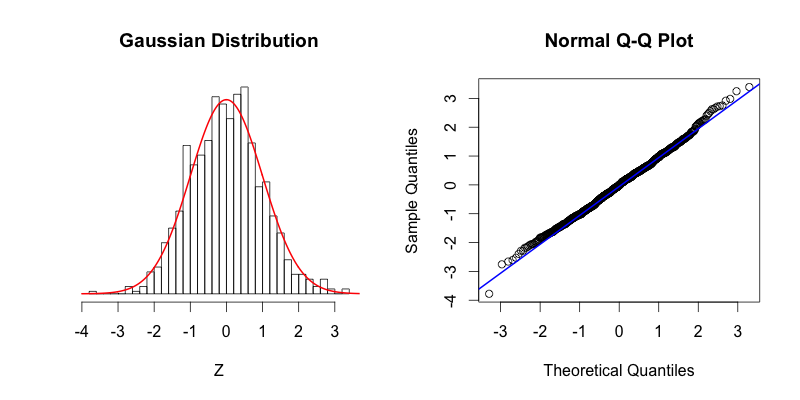
\includegraphics[width=0.7\linewidth]{gaussqq.png}
    \caption{Distribution normale et Q-Q plot pour la vérification de la normalité.}
    \label{fig:normality_check}
\end{figure}

\textbf{\(\checkmark\)} \textbf{Explication Mathématique:}
Le test de Shapiro-Wilk compare les statistiques d'ordre observées à celles attendues sous la loi normale. La statistique \( W \) est calculée comme suit:

\[
W = \frac{\left( \sum_{i=1}^{n} a_i x_i \right)^2}{\sum_{i=1}^{n} (x_i - \bar{x})^2}
\]

Où:
\begin{itemize}
    \item \( x_i \) est la \( i \)-ème statistique d'ordre,
    \item \( \bar{x} \) est la moyenne de l'échantillon,
    \item \( n \) est le nombre d'observations,
    \item \( a_i = \frac{m^T V^{-1}}{\sqrt{m^T V^{-1} V^{-1} m}} \), où \( m \) est le vecteur des quantiles théoriques et \( V \) la covariance.
\end{itemize}

\textbf{\(\checkmark\)} \textbf{Interprétation:}\\
\noindent \textbf{\(\rightarrow\)} \textbf{Valeur de \( W \)}: Plus proche de 1, meilleure est l'adéquation.\\
\textbf{\(\rightarrow\)} \textbf{p-value}: Si \( p < 0,05 \), les données ne sont pas normales; sinon, elles le sont.

\subsubsection*{Homoscédasticité (ou égalité des variances):}

L'homoscédasticité est cruciale avant d'appliquer des tests paramétriques. Le test de Levene compare les déviations absolues par rapport à la médiane pour évaluer l'égalité des variances entre groupes.

\textbf{\(\checkmark\)} \textbf{Hypothèses du Test:}\\
\noindent \textbf{\(\rightarrow\)} \( H_0 \): Les variances des groupes sont égales (homoscédasticité).
\textbf{\(\rightarrow\)} \( H_1 \): Les variances des groupes sont différentes (hétéroscédasticité).

\textbf{\(\checkmark\)} \textbf{Calcul des Déviations Absolues}:

Pour chaque observation \( x_{ij} \) dans le groupe \( j \):

\[
d_{ij} = \left| x_{ij} - \tilde{x}_j \right|
\]
Où \( \tilde{x}_j \) est la médiane du groupe \( j \).

\textbf{\(\checkmark\)} \textbf{ANOVA sur les Déviations Absolues:}

La statistique \( F \), qui compare la variance entre les groupes à celle intra-groupe, est donnée par:

\[
F = \frac{\text{Variance entre les groupes}}{\text{Variance intra-groupe}}
\]

Où:
\[
\text{Variance entre les groupes} = \frac{\sum_{j=1}^{k} n_j \left( \bar{d}_j - \bar{d} \right)^2}{k - 1}
\]
\[
\text{Variance intra-groupe} = \frac{\sum_{j=1}^{k} \sum_{i=1}^{n_j} \left( d_{ij} - \bar{d}_j \right)^2}{N - k}
\]

\textbf{\(\checkmark\)} \textbf{Interprétation des Résultats:}\\
\noindent \textbf{\(\rightarrow\)} \( F \) élevé indique des différences de variances entre les groupes.\\
\textbf{\(\rightarrow\)} \( p\text{-value} < 0{,}05 \): Rejet de H0, les variances sont différentes.\\
\textbf{\(\rightarrow\)} \( p\text{-value} \geq 0{,}05 \): H0 n'est pas rejetée, les variances sont homogènes.

\textbf{Autres conditions pour l’application des Tests paramétriques:}

\textbf{\(\checkmark\)} \textbf{Indépendance des observations}: Chaque observation doit être indépendante, sans influence d'une observation sur une autre.

\textbf{\(\checkmark\)} \textbf{Linéarité des relations}: Une relation est linéaire si elle suit une équation \( Y = aX + b \).

\noindent \textbf{\(\rightarrow\)} \textbf{Méthode des moindres carrés}: Pour vérifier la linéarité entre \( X \) et \( Y \), on ajuste un modèle de régression linéaire:

\[
Y = \beta_0 + \beta_1 X + \varepsilon
\]

Les coefficients \( \beta_0 \) et \( \beta_1 \) sont déterminés en minimisant la somme des carrés des résidus \( S(\beta_0, \beta_1) \):

\[
S(\beta_0, \beta_1) = \sum_{i=1}^{n} \left( Y_i - (\beta_0 + \beta_1 X_i) \right)^2
\]

\noindent \textbf{\(\rightarrow\)} \textbf{Dérivation pour minimisation}: Les dérivées partielles de \( S \) sont calculées pour minimiser cette fonction:

\[
\frac{\partial S}{\partial \beta_0} = -2 \sum_{i=1}^{n} \left( Y_i - (\beta_0 + \beta_1 X_i) \right)
\]
\[
\frac{\partial S}{\partial \beta_1} = -2 \sum_{i=1}^{n} X_i \left( Y_i - (\beta_0 + \beta_1 X_i) \right)
\]

\noindent \textbf{\(\rightarrow\)}  \textbf{Résolution des équations normales}:

\[
\beta_1 = \frac{n \sum_{i=1}^{n} X_i Y_i - \sum_{i=1}^{n} X_i \sum_{i=1}^{n} Y_i}{n \sum_{i=1}^{n} X_i^2 - \left( \sum_{i=1}^{n} X_i \right)^2}
\]
\[
\beta_0 = \frac{1}{n} \sum_{i=1}^{n} Y_i - \beta_1 \frac{1}{n} \sum_{i=1}^{n} X_i
\]

\noindent \textbf{\(\rightarrow\)}  \textbf{Coefficient de détermination \( R^2 \)}: Il mesure la proportion de la variance expliquée par le modèle:

\[
R^2 = 1 - \frac{\sum_{i=1}^{n} (Y_i - \hat{Y}_i)^2}{\sum_{i=1}^{n} (Y_i - \bar{Y})^2}
\]

\noindent \textbf{\(\rightarrow\)} \textbf{Interprétation de \( R^2 \)}:
\begin{itemize}
    \item \( R^2 = 1 \): Relation linéaire parfaite.
    \item \( R^2 = 0 \): Aucune relation linéaire.
\end{itemize}


\subsubsection{Test t de Student}

\textbf{Le test t (ou test de Student)} est utilisé pour comparer les moyennes de deux groupes ou d'un groupe par rapport à une valeur standard. Il vise à déterminer si les différences entre les moyennes sont statistiquement significatives ou dues au hasard.

\textbf{\(\checkmark\)} \textbf{Conditions d'application du test t:}\\
    \textbf{\(\rightarrow\)} \textbf{Normalité}: Les données doivent suivre une distribution normale.\\
    \textbf{\(\rightarrow\)} \textbf{Homogénéité}: Les variances des groupes doivent être égales.\\
    \textbf{\(\rightarrow\)} \textbf{Variables}: Comparaison d'une variable quantitative continue et d'une variable qualitative à deux groupes.\\
\textbf{\(\checkmark\)} \textbf{Hypothèses du test:}\\
    \textbf{\(\rightarrow\)} \( H_0 \): Les moyennes des deux groupes sont égales.\\
    \textbf{\(\rightarrow\)} \( H_1 \): Les moyennes des deux groupes sont différentes.\\

\textbf{\(\checkmark\)} \textbf{Formule du test t pour échantillons indépendants:}
\[
t = \frac{\bar{X}_1 - \bar{X}_2}{\sqrt{\frac{s_1^2}{n_1} + \frac{s_2^2}{n_2}}}
\]
Où:
\begin{itemize}
    \item \( \bar{X}_1 \) et \( \bar{X}_2 \) sont les moyennes des deux groupes.
    \item \( s_1^2 \) et \( s_2^2 \) sont les variances des deux groupes.
    \item \( n_1 \) et \( n_2 \) sont les tailles des échantillons.
\end{itemize}

\textbf{\(\checkmark\)} \textbf{Interprétation du test t:}\\
    \textbf{\(\rightarrow\)} \textbf{p-value \( < 0,05 \)}: Les différences entre les moyennes sont statistiquement significatives. On rejette \( H_0 \) et conclut que les moyennes sont différentes.\\
    \textbf{\(\rightarrow\)} \textbf{p-value \( \geq 0,05 \)}: Les différences ne sont pas significatives. On ne rejette pas \( H_0 \) et conclut qu'il n'y a pas suffisamment de preuves pour dire que les moyennes diffèrent.

\subsubsection{Test ANOVA}

    L'ANOVA (Analyse de Variance) est un test statistique permettant de comparer les moyennes de trois groupes ou plus. Contrairement au test de Levene, qui est utilisé pour tester l'homoscédasticité (égalité des variances) entre les groupes, l'ANOVA se concentre sur la comparaison des moyennes des groupes pour déterminer s'il existe des différences significatives.
    
\textbf{\(\checkmark\)} \textbf{Conditions d'application du test ANOVA:}\\
\textbf{\(\rightarrow\)} \textbf{Normalité}: Les données dans chaque groupe doivent suivre une distribution normale.\\
\textbf{\(\rightarrow\)} \textbf{Homogénéité des variances}: Les variances des groupes doivent être égales (homoscédasticité), ce que nous avons testé avec le test de Levene dans la section précédente.\\
\textbf{\(\rightarrow\)} \textbf{Variables}: Le test compare une variable quantitative continue (la réponse) avec une variable qualitative (les groupes).
    
\textbf{\(\checkmark\)} \textbf{Hypothèses du test:}\\
\textbf{\(\rightarrow\)} \( H_0 \): Les moyennes des groupes sont égales.\\
\textbf{\(\rightarrow\)} \( H_1 \): Au moins une des moyennes des groupes est différente.
    
    \textbf{\(\checkmark\)} \textbf{Formule du test ANOVA:}
    
    Nous avons déjà utilisé des formules similaires pour l'ANOVA appliqué aux déviations absolues dans le test de Levene pour évaluer l'homogénéité des variances. Dans ce contexte, l'ANOVA est utilisé pour comparer les moyennes des groupes en utilisant la même structure de calcul pour la statistique \( F \):
    
    \[
    F = \frac{\text{Variance inter-groupes}}{\text{Variance intra-groupes}}
    \]
    
Les formules spécifiques de la variance inter-groupes et intra-groupes ont déjà été introduites, mais ici elles servent à évaluer la différence \textbf{des moyennes}moyennes entre les groupes plutôt que leurs variances.
    
\textbf{\(\checkmark\)} \textbf{Interprétation des résultats:}\\
\textbf{\(\rightarrow\)}\textbf{ Si \( F \) est supérieur à la valeur critique}: On rejette \( H_0 \), ce qui indique qu'il existe une différence significative entre les moyennes des groupes.\\
\textbf{\(\rightarrow\)}\textbf{ Si \( F \) est inférieur ou égal à la valeur critique}: On ne rejette pas \( H_0 \), ce qui indique qu'il n'y a pas de différence significative entre les moyennes des groupes.
    
Ainsi, bien que l'ANOVA puisse être utilisé à la fois pour tester les variances (comme dans le test de Levene) et pour comparer les moyennes, son objectif principal dans cette section est d'examiner les différences de moyennes entre les groupes.    
    
\subsubsection{Test de Pearson}

\textbf{Le test de corrélation de Pearson} est un test statistique utilisé pour mesurer la force et la direction de la relation linéaire entre deux variables quantitatives continues. Le coefficient de corrélation de Pearson, noté \( r \), varie entre -1 et 1.

\textbf{\(\checkmark\)} \textbf{Conditions d'application du test de Pearson:}\\
    \textbf{\(\rightarrow\)} \textbf{Normalité}: Les deux variables doivent suivre une distribution normale.\\
    \textbf{\(\rightarrow\)} \textbf{Linéarité}: La relation entre les deux variables doit être linéaire.\\
    \textbf{\(\rightarrow\)} \textbf{Homogénéité (homoscédasticité)}: La variance des points doit être constante autour de la droite de régression.

\textbf{\(\checkmark\)} \textbf{Hypothèses du test de Pearson:}\\
    \textbf{\(\rightarrow\)} \( H_0 \): Il n’y a pas de corrélation linéaire entre les deux variables (\( r = 0 \)).\\
    \textbf{\(\rightarrow\)} \( H_1 \): Il existe une corrélation linéaire significative entre les deux variables (\( r \neq 0 \)).

\textbf{\(\checkmark\)} \textbf{Formule du coefficient de corrélation de Pearson:}\\
Le coefficient \( r \) est calculé à partir de la covariance des deux variables, divisée par le produit de leurs écarts-types:
\[
r = \frac{\sum_{i=1}^{n} (X_i - \bar{X})(Y_i - \bar{Y})}{\sqrt{\sum_{i=1}^{n} (X_i - \bar{X})^2} \sqrt{\sum_{i=1}^{n} (Y_i - \bar{Y})^2}}
\]
Où:
\begin{itemize}
    \item \( X_i \) et \( Y_i \) sont les valeurs des variables \( X \) et \( Y \).
    \item \( \bar{X} \) et \( \bar{Y} \) sont les moyennes de \( X \) et \( Y \).
    \item \( n \) est le nombre total d'observations.
\end{itemize}

\textbf{\(\checkmark\)} \textbf{Interprétation du coefficient \( r \):}\\
    \textbf{\(\rightarrow\)} \textbf{Si \( r \) est proche de 1 ou -1}: Cela indique une forte corrélation positive (1) ou négative (-1).\\
    \textbf{\(\rightarrow\)} \textbf{Si \( r \) est proche de 0}: Cela suggère qu’il n’y a pas de relation linéaire significative entre les deux variables.

\textbf{\(\checkmark\)} \textbf{Signification statistique du test de Pearson:}\\
La statistique \( r \) est comparée à une valeur critique, déterminée à partir de la distribution t avec \( n-2 \) degrés de liberté. Si la p-value associée est inférieure à 0,05, on rejette l'hypothèse nulle et on conclut qu'il existe une corrélation linéaire significative entre les deux variables.


\subsection{Tests non paramétriques}

Les \textbf{tests non paramétriques} sont utilisés lorsque les conditions des tests paramétriques ne sont pas respectées. Ils ne reposent pas sur des hypothèses strictes sur la distribution des données et sont adaptés aux petites tailles d'échantillon et aux données ordinales ou continues non normales.
\subsubsection{Test U de Mann-Whitney}

\textbf{Le test U de Mann-Whitney} est une alternative au test t de Student pour comparer deux groupes indépendants, lorsque les données ne suivent pas une distribution normale. Il se base sur \textbf{les rangs} des observations.

\textbf{\(\checkmark\)} \textbf{Conditions d'application:}\\
\textbf{\(\rightarrow\)} Les données doivent être ordinales ou continues.\\
\textbf{\(\rightarrow\)} Les groupes doivent être indépendants et les distributions non normales.

\textbf{\(\checkmark\)} \textbf{Principe des rangs:}\\
Les valeurs des deux groupes sont combinées et classées par ordre croissant. Chaque observation reçoit un rang correspondant à sa position.

\textbf{\(\checkmark\)} \textbf{Formule du test U:}
\[
U_1 = n_1 n_2 + \frac{n_1 (n_1 + 1)}{2} - R_1, \quad U_2 = n_1 n_2 + \frac{n_2 (n_2 + 1)}{2} - R_2
\]
Où \( n_1 \) et \( n_2 \) sont les tailles des groupes, et \( R_1 \) et \( R_2 \) les sommes des rangs.

La statistique \( U \) est le minimum de \( U_1 \) et \( U_2 \).

\textbf{\(\checkmark\)} \textbf{Interprétation:}\\
\textbf{\(\rightarrow\)} Si les rangs d'un groupe sont globalement plus élevés ou plus bas que ceux de l'autre, cela suggère une différence entre les groupes.\\
\textbf{\(\rightarrow\)} \textbf{p-value \( < 0{,}05 \)}: différence significative.\\
\textbf{\(\rightarrow\)} \textbf{p-value \( \geq 0{,}05 \)}: pas de différence significative.
    
\subsubsection{Test de Kruskal-Wallis}

\textbf{Le test de Kruskal-Wallis} est utilisé pour comparer trois groupes ou plus lorsque les données ne suivent pas une distribution normale. Il est une alternative à l'ANOVA.

\textbf{\(\checkmark\)} \textbf{Formule du test H:}
\[
H = \frac{12}{N(N+1)} \sum_{i=1}^{k} \frac{R_i^2}{n_i} - 3(N+1)
\]
Où:
\begin{itemize}
    \item \( N \) est le nombre total d'observations,
    \item \( R_i \) est la somme des rangs pour le groupe \( i \),
    \item \( n_i \) est la taille du groupe \( i \).
\end{itemize}

\textbf{\(\checkmark\)} \textbf{Interprétation du test H:}\\
    \textbf{\(\rightarrow\)} Si \( H \) est élevé, cela suggère des différences entre les groupes.\\
    \textbf{\(\rightarrow\)} Si la p-value \( < 0{,}05 \), les différences sont significatives.

\subsubsection{Test de Spearman}

\textbf{Le test de Spearman} mesure la force et la direction de la relation monotone entre deux variables ordinales ou continues non normales. Il est une alternative au test de Pearson pour les données non paramétriques.

\textbf{\(\checkmark\)} \textbf{Formule du coefficient de Spearman:}
\[
r_s = \frac{\sum_{i=1}^{n} (R_{x_i} - \frac{N+1}{2})(R_{y_i} - \frac{N+1}{2})}{\sqrt{\sum_{i=1}^{n} (R_{x_i} - \frac{N+1}{2})^2 \sum_{i=1}^{n} (R_{y_i} - \frac{N+1}{2})^2}}
\]
Où:
\begin{itemize}
    \item \( R_{x_i} \) et \( R_{y_i} \) sont les rangs des valeurs \( X \) et \( Y \),
    \item \( N \) est le nombre total d'observations.
\end{itemize}

\textbf{\(\checkmark\)} \textbf{Interprétation du coefficient de Spearman:}\\
    \textbf{\(\rightarrow\)} Si \( r_s \) est proche de 1 ou -1, la corrélation est forte.\\
    \textbf{\(\rightarrow\)} Si \( r_s \) est proche de 0, il n'y a pas de relation monotone.

\subsubsection{Test du Chi-Deux}

\textbf{Le test du Chi-Deux} est utilisé pour évaluer si les distributions observées dans des données catégorielles diffèrent des distributions attendues sous l'hypothèse d'indépendance entre les variables.

\textbf{\(\checkmark\)} \textbf{Calcul des fréquences attendues:}\\
Les fréquences attendues \( E_{ij} \) dans chaque cellule d'un tableau de contingence sont calculées en utilisant la formule:
\[
E_{ij} = \frac{R_i \times C_j}{N}
\]
Où:
\begin{itemize}
    \item \( R_i \) est le total de la \( i \)-ème ligne.
    \item \( C_j \) est le total de la \( j \)-ème colonne.
    \item \( N \) est le nombre total d'observations.
\end{itemize}

\textbf{\(\checkmark\)} \textbf{Formule du test du Chi-Deux:}\\
La statistique \( X^2 \) est calculée en comparant les fréquences observées aux fréquences attendues:
\[
X^2 = \sum_{i=1}^{r} \sum_{j=1}^{c} \frac{(O_{ij} - E_{ij})^2}{E_{ij}}
\]
Où:
\begin{itemize}
    \item \( O_{ij} \) est la fréquence observée dans la cellule \( (i, j) \),
    \item \( E_{ij} \) est la fréquence attendue dans la cellule \( (i, j) \).
\end{itemize}

\textbf{\(\checkmark\)} \textbf{Interprétation du test du Chi-Deux:}\\
    \textbf{\(\rightarrow\)} \textbf{Si la p-value \( < 0{,}05 \)}: Il existe une association significative entre les variables catégorielles.\\
    \textbf{\(\rightarrow\)} \textbf{Si la p-value \( \geq 0{,}05 \)}: Les variables sont indépendantes, c'est-à-dire qu'il n'y a pas de relation statistiquement significative entre elles.

\subsubsection{Test exact de Fisher}

\textbf{Le test exact de Fisher} est utilisé pour évaluer l'indépendance entre deux variables dans un tableau de contingence 2x2, particulièrement utile lorsque les effectifs sont petits ou les fréquences observées faibles.

\textbf{\(\checkmark\)} \textbf{Explication mathématique:}\\
Le test évalue la probabilité d'obtenir une répartition des données aussi extrême ou plus extrême que celle observée, sous l'hypothèse nulle d'indépendance.

Prenons un tableau de contingence 2x2:

\[
\begin{array}{|c|c|c|}
\hline
 & \text{Groupe 1} & \text{Groupe 2} \\
\hline
\text{Catégorie A} & a & b \\
\hline
\text{Catégorie B} & c & d \\
\hline
\end{array}
\]

Les probabilités des différentes configurations possibles sont calculées en respectant les totaux des lignes et colonnes (totaux marginaux) avec la distribution hypergéométrique:

\[
P = \frac{\binom{a+b}{a} \binom{c+d}{c}}{\binom{N}{a+c}}
\]

\textbf{\(\checkmark\)} \textbf{Interprétation de la p-valeur:}\\
\textbf{\(\rightarrow\)} Si la p-value \( < 0{,}05 \), on rejette l'hypothèse nulle d'indépendance.\\
\textbf{\(\rightarrow\)} Si la p-value \( \geq 0{,}05 \), les données sont compatibles avec l'indépendance entre les variables.

\section{Équilibrage des Classes avec SMOTE}

Dans le contexte de l'apprentissage supervisé, l'équilibrage des classes est crucial lorsqu'on traite des jeux de données déséquilibrés, c'est-à-dire lorsque certaines classes, souvent la classe minoritaire, sont sous-représentées. Le \textbf{SMOTE} (Synthetic Minority Over-sampling Technique) est une méthode avancée qui génère artificiellement de nouveaux exemples synthétiques pour la classe minoritaire, afin de rééquilibrer les données.

Le principe de SMOTE repose sur la génération de nouveaux points synthétiques en utilisant les données existantes des classes minoritaires. Le processus se fait comme suit:

\textbf{\(\rightarrow\)} \textbf{Étape 1:} Pour chaque exemple minoritaire \(x_i\), sélectionner un ou plusieurs \(k\)-voisins \(x_j\) dans la classe minoritaire, où \(j\) est un indice de voisin sélectionné parmi les plus proches voisins.
    
\textbf{\(\rightarrow\)} \textbf{Étape 2:} Générer un nouveau point \(x_{\text{new}}\) qui est situé quelque part sur la ligne reliant \(x_i\) et \(x_j\), selon la formule suivante:
    
    \[
    x_{\text{new}} = x_i + \delta \times (x_j - x_i)
    \]
    
    où \(x_i\) et \(x_j\) sont les points dans l'espace des features, et \(\delta\) est un facteur aléatoire compris entre 0 et 1.
    
\textbf{\(\rightarrow\)} \textbf{Étape 3:} Répéter ce processus pour plusieurs \(k\)-voisins afin de générer plusieurs points synthétiques, augmentant ainsi le nombre d'exemples dans la classe minoritaire.

\textbf{\(\checkmark\)} \textbf{Interprétation:}\\
\textbf{\(\rightarrow\)} \textbf{Utilité:} SMOTE permet de combler l'écart entre des exemples existants de la classe minoritaire et leurs voisins, créant ainsi des points synthétiques qui enrichissent la classe minoritaire tout en conservant les propriétés de l'espace des features.\\
\textbf{\(\rightarrow\)} \textbf{Impact:} Cette technique réduit les biais introduits par les classes déséquilibrées et améliore la performance des algorithmes de classification, notamment pour les classes minoritaires.

\textbf{\(\checkmark\)} \textbf{Détail du Calcul:}\\
\textbf{\(\rightarrow\)} \(x_i\): Un point dans la classe minoritaire.\\
\textbf{\(\rightarrow\)} \(x_j\): Un voisin \(k\)-proche de \(x_i\) dans la même classe minoritaire.\\
\textbf{\(\rightarrow\)} \(\delta\): Un nombre aléatoire entre 0 et 1, qui détermine la position du nouveau point sur la ligne reliant \(x_i\) et \(x_j\). Si \(\delta = 0.5\), \(x_{\text{new}}\) se situe au milieu de \(x_i\) et \(x_j\), tandis que des valeurs plus proches de 0 ou de 1 rapprochent \(x_{\text{new}}\) de \(x_i\) ou \(x_j\).

Cette méthode permet de créer de nouvelles observations synthétiques en comblant l'écart entre des points minoritaires et leurs voisins. Cela évite les biais liés aux données déséquilibrées sans simplement dupliquer les exemples existants, ce qui améliore les performances des modèles sans risquer de surapprentissage.

\section{Sélection des Caractéristiques (Feature Selection)}

La sélection des caractéristiques est une étape essentielle dans la construction de modèles de machine learning. Elle permet de réduire la dimensionnalité, d'améliorer la performance des modèles et de faciliter l'interprétation. 

\subsection{RFE (Recursive Feature Elimination)}

L'algorithme \textbf{RFE} (Élimination Récursive des Caractéristiques) sélectionne les caractéristiques les plus importantes en entraînant un modèle, en attribuant un poids à chaque caractéristique, puis en éliminant récursivement celles avec les poids les plus faibles.

\textbf{\(\checkmark\)} \textbf{Étape 1: Entraînement du modèle de base} \\ 
    Un modèle (comme une régression linéaire ou une forêt aléatoire) est entraîné sur l'ensemble des caractéristiques. Chaque caractéristique se voit attribuer un \textbf{poids} basé sur son influence sur les prédictions.

\textbf{\(\checkmark\)} \textbf{Étape 2: Élimination des caractéristiques moins importantes} \\ 
    Les caractéristiques ayant des poids proches de zéro ou jugées peu influentes sont éliminées.

\textbf{\(\checkmark\)} \textbf{Étape 3: Répétition du processus} \\ 
    L'algorithme répète le processus jusqu'à ce qu'il ne reste qu'un sous-ensemble optimal de caractéristiques.

Contrairement à la méthode des \textbf{Forêts Aléatoires} qui évalue l'importance via l'impureté des nœuds, \textbf{RFE} élimine les caractéristiques en se basant sur l'importance globale donnée par le modèle choisi. Cette approche est complémentaire à l'analyse d'importance, permettant d'affiner encore davantage le choix des caractéristiques.


\noindent \textbf{\(\rightarrow\)} \textbf{Utilité}: RFE est utile pour réduire la dimensionnalité tout en conservant les caractéristiques les plus influentes.\\
\textbf{\(\rightarrow\)} \textbf{Impact}: Cette méthode aide à éliminer les variables redondantes ou non pertinentes qui pourraient dégrader les performances des modèles.


\subsection{SelectKBest}

La méthode \textbf{SelectKBest} sélectionne les $k$ meilleures caractéristiques en fonction d'une mesure statistique. Un test statistique couramment utilisé est le test F, qui mesure le rapport entre la variance inter-classes et la variance intra-classes:

\[
F = \frac{\text{Variance entre les classes}}{\text{Variance intra-classes}}
\]

\noindent \textbf{\(\rightarrow\)} \textbf{Utilité}: Cette méthode est particulièrement utile pour sélectionner les caractéristiques ayant un fort pouvoir discriminant dans les modèles supervisés.\\
\textbf{\(\rightarrow\)} \textbf{Impact}: La sélection des caractéristiques en fonction du test F permet d'optimiser la performance des modèles en se concentrant sur les variables ayant une forte influence sur la variable cible.

\subsection{Feature Importance avec Forêt Aléatoire}

La \textbf{forêt aléatoire} est un ensemble d'arbres de décision qui attribue une importance à chaque caractéristique en fonction de la réduction d'impureté, mesurée par l'indice de Gini, aux nœuds de décision où la caractéristique est utilisée. L'importance d'une caractéristique est calculée en fonction de la somme de la réduction d'impureté avant et après la division.

La réduction de l'impureté, aussi appelée \textbf{réduction de Gini}, est définie par la formule:

\[
\Delta \text{Gini}(f) = \sum (\text{Gini avant} - \text{Gini après})
\]

\noindent \textbf{\(\rightarrow\)} \textbf{Utilité}: Cette méthode identifie les caractéristiques qui contribuent le plus à la séparation des classes dans un jeu de données complexe.\\
\textbf{\(\rightarrow\)} \textbf{Impact}: La forêt aléatoire est robuste aux interactions entre les caractéristiques, ce qui permet d'évaluer l'importance relative de chaque variable.

Le concept d'impureté et l'indice de Gini seront détaillés dans la partie consacrée aux \textit{modèles d'arbres de décision} dans la suite de ce chapitre.

\subsection{Conclusion}

Les trois algorithmes de sélection – RFE, SelectKBest et Feature Importance avec Forêt Aléatoire – sont complémentaires. RFE élimine les caractéristiques moins pertinentes, SelectKBest identifie statistiquement les meilleures, et la Forêt Aléatoire évalue leur importance via la réduction d'impureté. Ensemble, ces méthodes optimisent la sélection des variables, améliorant la performance des modèles.


\section{Modèles de Machine Learning}
Les modèles de machine learning permettent d’entraîner des algorithmes pour prédire des résultats en fonction des données. Ces algorithmes optimisent leurs paramètres internes pour minimiser les erreurs de prédiction.

\subsection{Régression Logistique}

\textbf{La régression logistique} est un modèle paramétrique utilisé principalement pour les tâches de classification binaire. Son objectif est de prédire la probabilité qu'une observation appartienne à une classe spécifique.

\textbf{\(\checkmark\)} \textbf{Concept Fondamental:}\\
La régression logistique modélise la probabilité qu’un événement se produise à l'aide d'une fonction sigmoïde. La formule de la probabilité est donnée par:

\[
P = \frac{1}{1 + e^{-(\beta_0 + \beta_1 x_1 + \dots + \beta_k x_k)}}
\]

Où:
\begin{itemize}
    \item \( P \): Probabilité que l'observation appartienne à la classe 1.
    \item \( \beta_0 \): Intercept (log-odds quand toutes les variables sont nulles).
    \item \( \beta_i \): Coefficients associés aux variables explicatives \( x_i \), qui déterminent l'importance de chaque variable.
    \item \( x_i \): Variables explicatives, ou caractéristiques, utilisées pour prédire la probabilité.
\end{itemize}

Le but est d’ajuster les coefficients \( \beta_0, \beta_1, \dots, \beta_k \) de manière à ce que le modèle prévoie correctement la classe à partir des données d'entrée.

\textbf{\(\checkmark\)} \textbf{Fonction de Coût (ou Perte):}\\
La fonction de coût dans un modèle de régression logistique est appelée \textbf{log-loss} ou \textbf{cross-entropy loss}. Elle mesure l’écart entre les prédictions du modèle et les vraies valeurs:

\[
L(\beta) = -\sum_{i=1}^{N} [y_i \log(p_i) + (1 - y_i) \log(1 - p_i)]
\]

Où:
\begin{itemize}
    \item \( N \): Nombre total d'observations dans le jeu de données.
    \item \( y_i \): Valeur réelle de la classe pour l'observation \( i \) (0 ou 1).
    \item \( p_i \): Probabilité prédite par le modèle pour l'observation \( i \).
\end{itemize}

La fonction de coût est essentielle, car elle guide l'algorithme sur la façon d'ajuster les coefficients du modèle pour mieux correspondre aux données observées.

\textbf{\(\checkmark\)} \textbf{Optimisation et Descente de Gradient:}\\
L’objectif de l’optimisation est de minimiser la fonction de coût en ajustant les coefficients \( \beta_0, \beta_1, \dots, \beta_k \). Une méthode populaire pour cela est la \textbf{descente de gradient}, où les coefficients sont mis à jour en suivant le gradient de la fonction de coût (qui indique la direction et l'intensité des modifications à apporter).

La mise à jour des coefficients se fait ainsi:
\[
\beta_i \leftarrow \beta_i - \alpha \frac{\partial L(\beta)}{\partial \beta_i}
\]

Où:
\begin{itemize}
    \item \( \alpha \) est le \textbf{taux d'apprentissage}, qui contrôle l'ampleur des mises à jour des coefficients.
    \item \( \frac{\partial L(\beta)}{\partial \beta_i} \) est le gradient de la fonction de coût par rapport à chaque coefficient \( \beta_i \).
\end{itemize}

Le \textbf{taux d'apprentissage} (\( \alpha \)) est un hyperparamètre important qui doit être bien choisi: un \( \alpha \) trop grand peut entraîner des oscillations, tandis qu'un \( \alpha \) trop petit rend l’apprentissage trop lent.
\subsubsection{Hyperparamètres}

Les \textbf{hyperparamètres} sont des variables définies avant l’entraînement du modèle. Contrairement aux coefficients \( \beta \), qui sont appris à partir des données, les hyperparamètres influencent le processus d'optimisation et de convergence du modèle.

\noindent \textbf{\(\rightarrow\)} \textbf{Taux d'apprentissage (\( \alpha \))}: Ce paramètre contrôle la taille des pas effectués pour ajuster les coefficients \( \beta \).

\noindent \textbf{\(\rightarrow\)} \textbf{Solver}: Le solver est l'algorithme utilisé pour minimiser la fonction de coût. Différents solveurs sont disponibles en fonction du type de problème et des contraintes de calcul. Voici un aperçu des principaux solveurs utilisés :

\begin{itemize}
    \item \textbf{Newton-CG}: Utilise la matrice Hessienne \( H \), qui contient les dérivées secondes de la fonction de coût, pour calculer la direction de descente. La mise à jour des coefficients \( \beta \) est effectuée comme suit:
    \[
    \beta \leftarrow \beta - H^{-1} \nabla L(\beta)
    \]
    Où \( H^{-1} \) est l'inverse de la Hessienne et \( \nabla L(\beta) \) est le gradient de la fonction de coût. Bien que précis, il peut être coûteux en temps pour les grands ensembles de données.

    \item \textbf{LBFGS} (Limited-memory Broyden–Fletcher–Goldfarb–Shanno): Version plus efficace de Newton-CG, LBFGS utilise les gradients récents au lieu de la matrice Hessienne complète pour estimer la direction de descente. La mise à jour est donnée par:
    \[
    \beta \leftarrow \beta - \alpha \cdot \text{Direction}
    \]
    LBFGS réduit la mémoire utilisée et accélère les calculs, ce qui le rend adapté pour les grands ensembles de données.

    \item \textbf{SAGA}: Améliore la descente de gradient stochastique (SGD) en combinant les gradients précédemment calculés pour affiner les mises à jour. La descente de gradient stochastique est une variante de la descente de gradient où les mises à jour des paramètres sont effectuées après chaque échantillon de données, plutôt que sur l'ensemble complet des données. Cela permet une convergence plus rapide, mais les mises à jour peuvent être plus bruyantes.

    SAGA combine cette approche avec un ajustement basé sur l'accumulation des gradients passés, offrant une meilleure stabilité et précision. La mise à jour des coefficients se fait ainsi:
    \[
    \beta \leftarrow \beta - \alpha \cdot \frac{1}{N} \sum_{i=1}^{N} \nabla L_i(\beta)
    \]
    Où \( \nabla L_i(\beta) \) est le gradient de la fonction de coût pour un échantillon \( i \), et \( N \) est la taille de l'ensemble de données.
\end{itemize}

\noindent \textbf{\(\rightarrow\)} \textbf{Max\_iter}: Définit le nombre maximal d'itérations de l'algorithme d'optimisation. Un nombre trop faible d'itérations peut entraîner une convergence incomplète, tandis qu'un nombre trop élevé peut augmenter le temps de calcul sans gains significatifs.

Ces hyperparamètres influencent la vitesse de convergence, la précision du modèle et la capacité d'adaptation aux données complexes.

\textbf{\(\checkmark\)} \textbf{Régularisation:}\\
La \textbf{régularisation} est un mécanisme qui ajoute une pénalité aux coefficients du modèle pour éviter le surajustement (overfitting). Il existe deux types principaux de régularisation:

\noindent \textbf{\(\rightarrow\)} \textbf{Régularisation L2 (Ridge)}: Ajoute une pénalité proportionnelle à la somme des carrés des coefficients pour éviter que certains coefficients ne deviennent trop grands. Sa formule est:
    \[
    L2 = \lambda \sum_{j=1}^{k} \beta_j^2
    \]
    Où \( \lambda \) contrôle l’importance de cette pénalisation.

\noindent \textbf{\(\rightarrow\)} \textbf{Régularisation L1 (Lasso)}: Pénalise la somme des valeurs absolues des coefficients, favorisant des modèles plus simples en mettant certains coefficients à zéro (ce qui peut exclure certaines variables inutiles):
    \[
    L1 = \lambda \sum_{j=1}^{k} |\beta_j|
    \]

Le choix de la régularisation dépend de l'objectif: L1 aide à la sélection des variables, tandis que L2 contrôle la taille des coefficients pour éviter le surajustement.

\textbf{\(\checkmark\)} \textbf{Résumé du Processus:}
\begin{enumerate}
    \item Initialisation des coefficients \( \beta_0, \dots, \beta_k \).
    \item Calcul de la fonction de coût en fonction des prédictions.
    \item Utilisation de l’algorithme de descente de gradient pour ajuster les coefficients en minimisant la fonction de coût.
    \item Application de la régularisation pendant l'optimisation pour éviter le surajustement.
    \item Répéter jusqu'à atteindre la convergence ou le nombre maximal d'itérations.
\end{enumerate}


\subsection{L’Arbre de Décision}

\textbf{\(\checkmark\)} \textbf{Concept Fondamental:}\\
Un arbre de décision classe des observations en les divisant en sous-groupes basés sur leurs caractéristiques. Chaque nœud interne pose une question, et les branches représentent les résultats des décisions, menant à des feuilles où la prédiction finale est réalisée.

\textbf{\(\checkmark\)} \textbf{Structure de l'Arbre:}\\
\textbf{Nœuds internes}: Posent des questions sur les caractéristiques.\\
\textbf{Branches}: Représentent les résultats des décisions.\\
\textbf{Feuilles}: Donnent la prédiction finale.

\textbf{\(\checkmark\)} \textbf{Processus de Division:}\\
L'arbre divise les données en sous-groupes aussi homogènes que possible, avec l'objectif de maximiser la pureté de chaque nœud.

\textbf{\(\checkmark\)} \textbf{Critères de Division:}\\
Les deux critères principaux pour mesurer la qualité des divisions sont l'Impureté de Gini et l'Entropie.

\textbf{1. Impureté de Gini:}\\
Mesure la pureté d’un nœud: un nœud est pur si toutes les observations appartiennent à la même classe. La formule est donnée par:

\[
Gini(S) = 1 - \sum_{k=1}^{K} P_k^2
\]

où \( P_k \) est la proportion d'éléments de la classe \( k \). Une réduction de l'impureté de Gini est calculée après chaque division:

\[
\Delta Gini = Gini(S) - Gini_{\text{moy}}
\]

La meilleure division est celle qui maximise la réduction de l'impureté.

\textbf{2. Entropie:}\\
L'entropie mesure l'incertitude des classes au sein d’un nœud. Plus l'entropie est faible, plus le nœud est homogène.

\[
Entropie(S) = -\sum_{k=1}^{K} P_k \log_2(P_k)
\]

\[
\Delta Entropie = Entropie(S) - Entropie_{\text{moy}}
\]

Le critère retenu dépend de la priorité donnée à la pureté des nœuds ou à la réduction de l'incertitude.

\textbf{Différence entre Gini et Entropie:}\\
Bien que similaires, Gini privilégie la pureté des nœuds, tandis que l’entropie est plus sensible aux classes rares. Les deux critères sont souvent utilisés de manière interchangeable selon les besoins du modèle.

\textbf{\(\checkmark\)} \textbf{Hyperparamètres:}\\
Pour éviter le surapprentissage, plusieurs hyperparamètres doivent être ajustés:\\
\noindent \textbf{\(\rightarrow\)} \textbf{Profondeur de l'arbre}: Limite la taille de l'arbre pour éviter la sur-optimisation.\\
\noindent \textbf{\(\rightarrow\)} \textbf{Max\_features}: Nombre de caractéristiques considérées à chaque division.\\
\noindent \textbf{\(\rightarrow\)} \textbf{min\_samples\_split} et \textbf{min\_samples\_leaf}: Limites pour diviser un nœud ou créer une feuille.

\textbf{\(\checkmark\)} \textbf{Optimisation:}\\
Des méthodes comme \textbf{RandomizedSearchCV} permettent de tester différentes combinaisons d’hyperparamètres pour obtenir le meilleur modèle. Contrairement à \textbf{GridSearchCV}, qui explore de manière exhaustive toutes les combinaisons possibles, \textbf{RandomizedSearchCV} sélectionne aléatoirement un sous-ensemble de ces combinaisons.

\noindent \textbf{\(\rightarrow\)} \textbf{Principe}: \textbf{RandomizedSearchCV} effectue un échantillonnage aléatoire des combinaisons d'hyperparamètres à tester. Au lieu de tester toutes les possibilités, il en sélectionne une fraction aléatoire, ce qui permet de trouver une solution optimale plus rapidement, particulièrement utile pour les grands jeux de données ou lorsque le nombre d'hyperparamètres à ajuster est important.

\noindent \textbf{\(\rightarrow\)} \textbf{Différence avec GridSearchCV}: \textbf{GridSearchCV} explore systématiquement chaque combinaison d’hyperparamètres, tandis que \textbf{RandomizedSearchCV} teste aléatoirement un certain nombre d'échantillons, ce qui permet une optimisation plus rapide.

\textbf{Note:} La fonction de coût et les détails sur la descente de gradient, souvent utilisés dans l’optimisation d’hyperparamètres, ont déjà été abordés dans une section précédente.

\textbf{\(\checkmark\)} \textbf{Résumé du Processus:}\\
L'arbre de décision divise les données en sous-groupes en fonction des caractéristiques, en utilisant les critères de Gini ou d’entropie pour maximiser la pureté à chaque division. Les hyperparamètres contrôlent la complexité du modèle, garantissant un bon équilibre entre précision et généralisation.

\subsection{La Forêt Aléatoire: un modèle non paramétrique}

\textbf{\(\checkmark\)} \textbf{Concept Fondamental:}\\
La forêt aléatoire est un ensemble d'arbres de décision, où plusieurs arbres sont créés à partir d'échantillons différents des données. Chaque arbre effectue sa propre prédiction, et les résultats sont combinés pour améliorer la précision globale. Ce processus réduit le surapprentissage et améliore la robustesse du modèle.

\textbf{\(\checkmark\)} \textbf{Création des Arbres de Décision:}
\begin{enumerate}
    \item \textbf{Échantillonnage Bootstrap:} Chaque arbre est formé à partir d’un sous-échantillon aléatoire avec remplacement (bootstrap) des données d’entraînement. Cela permet de diversifier les arbres créés, réduisant le risque de surajustement (overfitting).
    
    \item \textbf{Sélection Aléatoire des Caractéristiques:} À chaque nœud, une fraction aléatoire des caractéristiques est sélectionnée pour déterminer les divisions, ce qui diminue la corrélation entre les arbres et favorise une meilleure généralisation.

    \item \textbf{Vote Majoritaire:} Chaque arbre vote pour une classe, et la classe finale prédite est celle qui reçoit le plus de votes. Cela est formalisé par l'équation suivante:
    \[
    \hat{y} = \arg\max_k \left( \sum_{i=1}^{T} \mathbf{1}(\hat{y}_i = k) \right)
    \]
    où \( T \) est le nombre total d'arbres et \( k \) les classes possibles.
\end{enumerate}

\textbf{\(\checkmark\)} \textbf{Optimisation des Hyperparamètres:}\\
La performance d'une forêt aléatoire dépend fortement de la configuration de ses hyperparamètres. Voici quelques hyperparamètres clés à ajuster:\\
\noindent \textbf{\(\rightarrow\)} \textbf{n\_estimators:} Nombre d’arbres dans la forêt. Plus il est élevé, meilleure est la précision, mais cela augmente le temps de calcul.\\
\noindent \textbf{\(\rightarrow\)} \textbf{max\_features:} Nombre de caractéristiques à considérer pour chaque division. Une valeur courante est la racine carrée du nombre total de caractéristiques.\\
\noindent \textbf{\(\rightarrow\)} \textbf{min\_samples\_split:} Nombre minimum d’échantillons requis pour diviser un nœud. Ajuster ce paramètre permet de contrôler la profondeur des arbres.\\
\noindent \textbf{\(\rightarrow\)} \textbf{oob\_score (out-of-bag score):} Ce score est calculé en utilisant les échantillons non sélectionnés par bootstrap pour entraîner un arbre. Il permet d’évaluer la performance du modèle sans avoir recours à une validation croisée, économisant ainsi du temps de calcul.

\textbf{\(\checkmark\)} \textbf{Importance des Caractéristiques:}\\
La forêt aléatoire permet également de mesurer l'importance des caractéristiques en évaluant leur contribution à la réduction de l'impureté (Gini ou entropie) aux nœuds de décision. Les détails sur le calcul de l'importance des caractéristiques ont déjà été abordés dans la section dédiée à la sélection des caractéristiques. Ici, nous rappelons que cette importance est calculée en fonction de la réduction d'impureté à chaque nœud où une caractéristique est utilisée.

\textbf{\(\checkmark\)} \textbf{Relation avec l'Arbre de Décision:}\\
Contrairement à un arbre de décision unique, la forêt aléatoire utilise plusieurs arbres créés à partir de différentes sous-parties des données et des caractéristiques. Cette approche réduit le surapprentissage, rendant le modèle plus robuste. L'agrégation des prédictions améliore la capacité du modèle à capturer la variabilité des données, produisant ainsi des résultats plus précis et plus généralisables.

\subsection{AdaBoost: Amélioration des Arbres de Décision}

\textbf{\(\checkmark\)} \textbf{Concept Fondamental:}\\
AdaBoost est une technique de \textbf{boosting} qui améliore les performances des arbres de décision en créant des modèles séquentiels. Contrairement à la forêt aléatoire qui utilise des arbres indépendants, le boosting corrige les erreurs des arbres précédents, rendant le modèle plus précis à chaque étape.

\textbf{AdaBoost} se concentre sur les observations mal classées en attribuant des poids plus importants à ces données après chaque itération. L’objectif est de forcer les arbres suivants à prêter plus d’attention à ces erreurs.

\textbf{\(\checkmark\)} \textbf{Explication du Processus:}
\begin{enumerate}
    \item \textbf{Poids des observations:} Chaque observation a un poids. Initialement, toutes les observations ont le même poids.
    \item \textbf{Ajustement des poids après chaque itération:} Les observations mal classées reçoivent des poids plus élevés afin que l’arbre suivant se concentre davantage sur ces erreurs.
\end{enumerate}

La formule suivante détermine les poids des modèles faibles \( \alpha_m \) selon les erreurs (\( \epsilon_m \)):
\[
\alpha_m = \frac{1}{2} \log\left(\frac{1 - \epsilon_m}{\epsilon_m}\right)
\]
Les poids des observations sont ensuite mis à jour:
\[
w_{i,m+1} = w_{i,m} \exp(-\alpha_m y_i h_m(x_i))
\]
Cela permet aux arbres suivants de mieux corriger les erreurs des arbres précédents.

\textbf{\(\checkmark\)} \textbf{Utilité Pratique:}\\
AdaBoost est particulièrement utile lorsque l’on veut se concentrer sur les observations difficiles à classer. Il est efficace pour les ensembles de données où certaines erreurs sont difficiles à corriger avec des méthodes traditionnelles.

\textbf{\(\checkmark\)} \textbf{Hyperparamètres:}\\
\noindent \textbf{\(\rightarrow\)} \textbf{n\_estimators}: Nombre d’arbres. Un nombre élevé permet d’améliorer la précision, mais au prix d’un temps de calcul plus long.\\
\noindent \textbf{\(\rightarrow\)} \textbf{learning\_rate}: Il détermine la contribution de chaque nouvel arbre aux prédictions finales. Un faible taux d’apprentissage (par exemple, 0,1) est souvent recommandé pour une meilleure convergence.\\
\noindent \textbf{\(\rightarrow\)} \textbf{max\_depth}: La profondeur maximale des arbres. Une profondeur plus faible permet d’éviter le surajustement.\\
\noindent \textbf{\(\rightarrow\)} \textbf{oob\_score}: L’utilisation des échantillons hors sac (out-of-bag) permet d’évaluer la performance sans validation croisée.

\textbf{\(\checkmark\)} \textbf{Résumé du Processus:}
\begin{enumerate}
    \item \textbf{Initialisation:} Démarrage avec des poids égaux.
    \item \textbf{Correction des erreurs:} Chaque arbre suivant est formé pour corriger les erreurs du modèle précédent.
    \item \textbf{Mise à jour des prédictions:} Les poids sont ajustés, et le modèle est mis à jour à chaque itération.
    \item \textbf{Ajustement des hyperparamètres:} Des hyperparamètres tels que le taux d’apprentissage et la profondeur des arbres sont ajustés pour maximiser la performance tout en évitant le surajustement.

\end{enumerate}

\textbf{\(\checkmark\)} \textbf{Conclusion:}\\
AdaBoost exploite la séquence et l’adaptation dans la formation des arbres en se concentrant sur les erreurs les plus difficiles à corriger. Cela permet d’améliorer significativement les performances des modèles d’arbres de décision, surtout dans les ensembles de données où certaines observations sont particulièrement difficiles à classer.

\subsection{Conclusion}
Les modèles de machine learning présentés offrent diverses approches pour la classification et la régression. L'optimisation des hyperparamètres, comme la validation croisée et le réglage de \( C \) et \( \gamma \), ajuste les modèles pour améliorer la précision et éviter le surapprentissage.

\section{Deep Learning}

Dans cette section, nous nous concentrons sur les aspects techniques et mathématiques des réseaux de neurones profonds. on va explorer comment les couches de neurones, les fonctions d'activation, et les processus d'entraînement tels que la \textbf{backpropagation} et la descente de gradient sont mis en œuvre pour optimiser les modèles d'apprentissage.

\subsection{Les Couches dans un Réseau de Neurones}

Un réseau de neurones profond est composé de plusieurs couches. Chaque couche réalise une transformation linéaire suivie d'une fonction d'activation non linéaire. Mathématiquement, une couche \( l \) applique la transformation suivante:

\[
h^{(l)} = f(W^{(l)} h^{(l-1)} + b^{(l)})
\]

Où:
\begin{itemize}
    \item \( h^{(l-1)} \) est le vecteur de sortie de la couche précédente (ou les entrées pour la première couche),
    \item \( W^{(l)} \) est la matrice des poids de la couche \( l \),
    \item \( b^{(l)} \) est le biais de la couche \( l \),
    \item \( f \) est la fonction d'activation appliquée à chaque neurone.
\end{itemize}

Cette formule montre comment chaque neurone d'une couche reçoit une combinaison pondérée des neurones de la couche précédente, plus un biais, puis passe cette somme à travers une fonction d'activation.
\subsection{Fonctions d'Activation}

Les fonctions d'activation ajoutent de la non-linéarité, permettant aux réseaux d'apprendre des relations complexes.

\textbf{\(\checkmark\)} \textbf{ReLU:} 
\[ f(x) = \max(0, x) \]
ReLU renvoie \( x \) si \( x \) est positif, sinon 0, accélérant l'apprentissage. Toutefois, certains neurones peuvent cesser d'apprendre si leurs valeurs deviennent constamment nulles.

\textbf{\(\checkmark\)} \textbf{Tanh:} 
\[ f(x) = \frac{e^x - e^{-x}}{e^x + e^{-x}} \]
Tanh produit des sorties entre -1 et 1, utile pour centrer les données, mais entraîne la saturation des gradients pour des valeurs extrêmes, ralentissant l'apprentissage.

\textbf{\(\checkmark\)} \textbf{Sigmoïde:} 
\[ f(x) = \frac{1}{1 + e^{-x}} \]
La Sigmoïde compresse entre 0 et 1, idéale pour la classification binaire, mais ralentit l'apprentissage dans les réseaux profonds en réduisant les gradients pour des valeurs extrêmes de \( x \).


\subsection{Entraînement et Backpropagation}

L'entraînement d'un réseau de neurones consiste à ajuster les poids et les biais pour minimiser une fonction de perte. Ce processus est réalisé via l'algorithme de \textbf{backpropagation}, en conjonction avec des méthodes d'optimisation comme la \textbf{descente de gradient}.

\subsubsection{Calcul de la Fonction de Perte}

La fonction de perte mesure l'écart entre la sortie prédite et la valeur réelle. Dans les tâches de classification binaire, une fonction courante est la \textbf{binary cross-entropy}, définie comme suit:

\[
L(\hat{y}, y) = - \frac{1}{N} \sum_{i=1}^{N} \left[ y_i \log(\hat{y}_i) + (1 - y_i) \log(1 - \hat{y}_i) \right]
\]

Où:
\begin{itemize}
    \item \( N \) est le nombre d'exemples dans le lot (batch),
    \item \( y_i \) est la vraie classe de l'exemple \( i \) (soit 0, soit 1),
    \item \( \hat{y}_i \) est la probabilité prédite par le modèle que l'exemple \( i \) appartienne à la classe 1.
\end{itemize}

\subsubsection{Backpropagation et Descente de Gradient}

Une fois la perte calculée, l'algorithme de \textbf{backpropagation} est utilisé pour propager l'erreur depuis la couche de sortie jusqu'aux couches précédentes afin de calculer les gradients des poids et des biais. 

L'objectif est de minimiser la fonction de perte \( L \). Pour ce faire, on ajuste les poids \( W \) et les biais \( b \) en utilisant la descente de gradient:

\[
W_{\text{nouveau}} = W_{\text{ancien}} - \eta \frac{\partial L}{\partial W}
\]
\[
b_{\text{nouveau}} = b_{\text{ancien}} - \eta \frac{\partial L}{\partial b}
\]

Où:
\begin{itemize}
    \item \( \eta \) est le taux d'apprentissage, qui contrôle la taille des pas de mise à jour,
    \item \( \frac{\partial L}{\partial W} \) et \( \frac{\partial L}{\partial b} \) sont les gradients de la perte par rapport aux poids et aux biais.
\end{itemize}

Les gradients sont calculés en utilisant la règle de la chaîne pour rétropropager l'erreur depuis la couche de sortie vers les couches cachées. Cela permet à chaque neurone d'ajuster ses poids en fonction de sa contribution à l'erreur totale.

\subsection{Régularisation et Dropout}

La \textbf{régularisation \( L_2 \)} aide à prévenir le surapprentissage en ajoutant une pénalité proportionnelle à la somme des carrés des poids à la fonction de perte :

\[ 
L_{\text{rég}} = L + \lambda \sum_{i} W_i^2 
\]

Cela empêche certains neurones de développer des poids trop élevés, réduisant ainsi la spécialisation excessive du modèle.

Le \textbf{Dropout}, autre technique courante, désactive aléatoirement un pourcentage de neurones à chaque itération, empêchant leur co-adaptation excessive. Mathématiquement, pour un neurone \( h^{(l)} \) dans la couche \( l \) :

\[
h^{(l)} = \text{Dropout}(f(W^{(l)} h^{(l-1)} + b^{(l)}))
\]

Le taux de Dropout, un hyperparamètre clé, doit être bien ajusté : un taux trop bas a peu d'effet, tandis qu'un taux trop élevé peut entraîner un sous-apprentissage.

\subsection{Hyperparamètres: Signification et Impact}
Les hyperparamètres, comme expliqué précédemment, sont des variables fixées avant l'entraînement. Voici les principaux hyperparamètres et leur impact:
\begin{itemize}
\item \textbf{Nombre d'époques:} Nombre de passages complets sur l'ensemble de données. Trop peu entraîne un sous-apprentissage, trop d'époques peut entraîner un surapprentissage.

\item \textbf{Taille du Batch:} Nombre d'exemples utilisés par itération. Petits batchs = mises à jour plus fréquentes et bruitées. Grands batchs = plus stables mais nécessitent plus de mémoire.

\item \textbf{Dropout Rate:} Proportion de neurones désactivés à chaque itération. Taux élevé réduit le surapprentissage, mais trop élevé risque de sous-apprentissage.

\end{itemize}

\subsection{Conclusion}

Le deep learning transforme les données à travers des couches non linéaires. L'optimisation par backpropagation ajuste les poids pour minimiser la perte. La régularisation, le dropout, et l'ajustement des hyperparamètres évitent le surapprentissage et améliorent les performances.

\section{Interprétation des Modèles pour la Prédiction de la Satisfaction Client}

Une fois les modèles prédictifs validés, il est essentiel d'interpréter les résultats pour identifier les profils clients les plus satisfaits. L'algorithme de clustering KMeans est utilisé pour regrouper les clients en groupes homogènes, puis nous calculons la probabilité de satisfaction pour chaque groupe.

\subsection{Clustering avec KMeans}

KMeans est une méthode non supervisée qui partitionne les observations en \(k\) clusters en minimisant les distances intra-clusters. L'objectif est de former des groupes où les observations sont proches du centroïde (centre) du cluster.

\textbf{Formulation mathématique:}

L'algorithme minimise l'inertie intra-cluster:

\[
\min \sum_{i=1}^{k} \sum_{x \in C_i} \| x - \mu_i \|^2
\]

où \( C_i \) est le \(i\)-ème cluster, \( x \) une observation, \( \mu_i \) le centroïde, et \( \| x - \mu_i \|^2 \) la distance euclidienne au carré.\\
\textbf{Étape 1}: Chaque observation est assignée au cluster le plus proche.\\
\textbf{Étape 2}: Les centroïdes sont recalculés en prenant la moyenne des observations assignées. Ce processus se répète jusqu'à convergence.

\subsection{Calcul de la Probabilité de Satisfaction}

Chaque cluster représente un groupe distinct de clients. Pour chaque cluster \( C_i \), la probabilité moyenne de satisfaction est calculée par:

\[
P_{\text{satisfaction}}(C_i) = \frac{1}{|C_i|} \sum_{x \in C_i} P_{\text{satisfaction}}(x)
\]

où \( P_{\text{satisfaction}}(x) \) est la probabilité de satisfaction de chaque client \( x \), et \( |C_i| \) est la taille du cluster. Cela permet d'identifier les groupes de clients les plus satisfaits.

\subsection{Interprétation des Résultats}

L'analyse des résultats permet d'identifier les caractéristiques communes des clients dans les clusters avec la plus forte probabilité de satisfaction. Par exemple, cela peut révéler des segments de clients ayant des habitudes de consommation spécifiques.

\subsection{Conclusion}

L'algorithme KMeans identifie des groupes homogènes de clients et, en calculant la probabilité de satisfaction pour chaque cluster, permet de dégager des profils types. Cela fournit une vision claire des segments de clientèle à cibler, en se basant sur les caractéristiques des clients les plus satisfaits.

\section{Conclusion}

Ce chapitre a présenté des outils essentiels pour le prétraitement des données, l’analyse de corrélation et la modélisation. Grâce à des méthodes comme SMOTE, la sélection des caractéristiques et des modèles de machine learning, nous avons établi des bases solides pour optimiser la précision et la robustesse des modèles prédictifs.
